\chapter{Evaluation}
\label{chap:eval}

This section relates to the evaluation of various aspects of the project.  The Src researcher whom the project focused around was off on maternity leave for the duration of this phase of the project so no evaluations were able to be performed with them.

\section{First Evaluation}

The first evaluation in the second phase of the project occurred in November 2013.  The user group was made up of two biologists.  One who had taken part in the first evaluation meeting and one person who had no knowledge of the project.

\subsection{User Group}

As the domain expert was not available, insight based evaluation was unable to be used.  A more traditional approach had to be taken.  Before the evaluation  a typical scenario that a user might encounter was prepared.  The task was to open a file, annotate it and run the animation visualisation, and attach supporting documentation.  The task was prepared at two levels of instruction.  The first level was a paragraph of text that described what was to be done.  The second level was a step-by-step list of instructions to perform.  The user group was observed as they attempted the task and were offered assistance when required.  Afterwards the user group was given a questionnaire to fill in about their experience. After filling in the questionnaire there was a discussion on their answers and any further thoughts that they had.

The task was prepared at two levels to try and gauge how easy the program is to use.  The users were first presented with the textual description and if they had been unable to complete the task with this then they would have been given the step-by-step instructions instead.  The users were able to complete the task from the textual description alone.  This is a good sign that the new tool is usable.

Some issues were encountered:

\begin{itemize}
\item The users were unfamiliar with MacOS -- Both users were unable to locate the menu bar as it is not attached to the program as in Windows.  Future evaluations will use Windows.
\item The users were unclear as to what was going to happen when annotating.  When annotating the graph with an arrow the user had to click twice to place it but there was no indication of this, nor was it clear to them which way the arrow would be drawn.  This has now been fixed. Different cursors are used to give feedback to the user that they should click, and rather than just relying on two clicks with no information as to where the arrow is going to point, after the first click (which places the tail of the arrow) an arrow will be drawn that follows the cursor until the second click placing the annotation.
\item Lack of ability to edit, move, or delete annotations -- Once an annotation was placed it was there permanently.  The ability to edit annotations was always planned, but had not been implemented in time.  But the amount of frustration it gave the users was very high.  It was a principle in all three of Norman~\cite{normsev}, Neilson~\cite{neilten} and Schniederman's~\cite{shgold} lists that a user should be able to fix mistakes.  Since the evaluation, editing and deleting of annotations has been implemented.  This means any mistakes can be corrected.
\item Initially the users were confused by what all the buttons on the matplotlib toolbar did.  After discovering the tooltips, and seeing what effect the buttons had, they were comfortable with them.  If a user were to do something they did not intend they are able to undo it. All the matplotlib built-in buttons on the toolbar can be undone and redone from the toolbar.  Any buttons implemented for this tool are covered by the undo and redo functionality implemented across the whole program.  Being able to recover from their actions on the toolbar means no hindrance to discovery and so needs no further action.  It would be desirable to have the two undo methods unified but a way to do this could not be found.
\item The users were confused by some of the terminology.  In particular the could not distinguish between ``save graph'' and ``save model''. These items in the menu have now been grouped more carefully to help the user distinguish them.  A related issue was worrying that ``save graph'' was going to override the results file.  To rectify this the menu items that create new files have been renamed ``export ...''.
\item The users struggled to start a new session.  When asked for a title they did not know what the title was going to be used for.  When trying to add files, rather than use the add files button in the dialogue, they tried to use the file menu.  Having two routes into the visualisation seemed to be confusing them.  Now the file menu open file has been removed.  To create a visualisation the user has to go through the new session wizard.
\item When placing species in the cell one of the users did not understand what they were being asked to do.  One of the users did understand.  To fix this user input has been removed from the process.  The species locations are parsed automatically from the model.  This has required the model file to be added to the session by the user.
\item They liked the animation feature and thought it would be very useful (One of the users did their PhD in transport and expressed a desire to have had this feature during the PhD).  They did feel that it wouldn't be useful directly for papers, but that it would be useful when deciding what to include in a paper.
\item One of the users asked if there was a map of the cell.  When presented with the model visualisation they thought that it did look nice, but they were unsure of its usefulness.  The model viewing has since been merged into the animation visualisation.
\item The results from the questionnaire indicated that both users thought the tool's appearance was good.  The tool was average in difficulty to use -- neither easy nor difficult. The annotation buttons on the toolbar were clear as to what they did. It was obvious how to attach supporting files.  Both users thought that it is very useful to attach files to the session so that they can be easily emailed to a colleague.  They thought it would be useful to have the graph automatically annotated, but they wanted to the ability to disable any automatic annotations.  Both users found the animation useful.
\end{itemize}

\subsection{Personal}

At this stage in the development the program was in a state where some existing functionality had been broken.  This had not been noticed during development.  This highlighted architectural flaws in the code.  There were multiple paths through the program that data was taking.  Code was also duplicated across the program.  Since then a majority of these bugs have been ironed out and the duplications removed. The code is now better architected.  At the time of the evaluation with the users not all the features could be tested with them -- mainly the plot preferences dialogue.  These features have now been fixed and they will be evaluated by the users at the next meeting.

Having the users use the program has also highlighted a number of usability problems: menus being badly organised and named, features such as annotation rely on assumed knowledge to work them.  All this created an unfriendly environment for the user.  This was due to losing sight of the need for usability during development and when testing new features not removing the knowledge of the code from my mind.  Since this evaluation the three lists of usability~\cite{shgold}\cite{normeval}\cite{neilten} have been refocused on and the code gone through and the principles applied.

The positive feedback on animation and annotation, two of the core new features, is excellent validation of the new work.

\section{Evaluation 2 - Start of Second Semester}

The second evaluation in the second phase of the project occurred in February 2014.  There were two evaluations this time.  One with the same group of biologists as before and another with an Informatics researcher who uses Bio-PEPA.

Since the last evaluation work had been done to fix the issues encountered since the last time and two new features had been added: annotation of the animation and data normalisation and export.

\subsection{User Group}

As with the first evaluation a task was prepared at two levels of instruction.  Afterwords the users were given a questionnaire to fill in.  They were also given a chance to use the program without following a task, giving them a chance to explore.  Again, after the questionnaire a discussion was held.

The findings of the evaluation were as follows:

\begin{itemize}
\item There were inconsistencies in the text giving instructions to the user.  This did not appear to cause confusion, but it was noticed by both of the users.  This was fixed.  All the user facing text in the project was checked and changed if necessary.
\item The users kept trying to drag annotations on the graph after creation. The users wanted to be able to drag the annotation to a new position to fine-tune the position.  They attempted to do this by left clicking on the annotation and dragging it.  This issue has not been solved.  Currently if the user places an annotation in the wrong location they can delete the annotation and put a new one in the correct place.  For the user this is not the most desirable solution, but it was felt that the time could be better spent in other areas of the project.  This would, hopefully, be implemented in future work.
\item The users found the new model visualisation much more informative.  This is a positive as the reason for implementing model visualisation was to help the users understand what happens in the model more.  The users did however think that adding in labels of the compartments would be useful as they may not be familiar with the model.  The labelling of compartments has since been implemented.
\item The users found the task to be easy to complete.  This is a good result.  The tool needs to be easy to use.  They did not give full marks for ease, so there is still room for improvement.
\item The users found it much easier to start a new session using the wizard.  This was a task they had struggled with during the previous evaluations.  There were still aspects that they did not discover such as being able to select multiple files.  Guidance text has since been added to the wizard pages.
\item The users indicated that they found annotating animations easy and intuitive.  This is positive.  It is a new feature and the users indicated little need for change.
\item The users uncovered some bugs in the system.  The bugs included: not all types of annotations being able to be placed on the plot and the colours of the cell segments not being updated after changing the colour of the line.  All bugs discovered have since been fixed.
\item The users were very much in favour of being able to use plots as queries.  This provided justification for pursuing it as a project goal.
\item The users were very much in favour of being able to collaborate in real time. This provided justification for pursuing it as a project goal.
\item The users found it easy to normalise \& export the data and indicated that they thought it would be a useful feature to have.
\item The users were pleased by the addition of undo functionality.  They appeared to be much more willing to make mistakes knowing that they could undo their mistakes.
\item The users were pleased that since the last evaluation the ability to modify and delete annotations had been added.
\end{itemize}

\subsection{Bio-PEPA Developer}

The evaluation with the Bio-PEPA developer was similar to the evaluation with the user group.  The developer was given the same task and after performing the task there was a discussion about their performance and their feelings about the tool.

\begin{itemize}
\item It was not clear to the user what the new model visualisation was displaying.  This has been solved by adding text to the model visualisation page explaining what the user is seeing.
\item The user uncovered a bug in how annotations are rendered when the graph is viewed with the data normalised.  The problem and the solution are discussed in Section~\ref{sec:annotation_graph}.
\end{itemize}

\subsection{Personal}

The results from this evaluation were positive.  The users seemed much more comfortable using the tool.  This was hopefully down to the efforts made to improve the usability.  There are still too many bugs being discovered by the users.  This was addressed by spending a significant amount of time on tracking down and fixing bugs.  The positive reception to the ideas for plots as queries and real time collaboration led to them being added as project goals.

\section{Evaluation 3 - End of Second Semester}

The third and final evaluation in the second phase of the project occurred in March 2014.  There were two evaluations this time.  These were the same as the previous evaluation: the user group and an Informatics researcher who uses Bio-PEPA.  Given that this was the final evaluation a further focus was placed on evaluating the users preferences between this new tool and the Eclipse plugin.

Since the previous evaluation a sizeable amount of work had gone into improving the stability.  The new features that had been added were plots as queries and real time collaboration.  These were unable to be evaluated by the users. Plots as queries could not be evaluated as it has not been tied into the \ac{UI}.  Real time collaboration could not be evaluated with the users as it would have required another laptop.  The layout of the program had changed and this was tested by the users.

\subsection{User Group}

Like the other evaluations the users were given a task to complete.  Afterwards there was a questionnaire and a discussion.

The findings are as follows:

\begin{itemize}
\item The users liked the appearance of the tool.  Since the previous evaluation significant effort had been placed into making the user interface more aesthetically pleasing.  The users strongly preferred the new \ac{UI}.  This justifies the effort into the \ac{UI}.
\item The users indicated that they found the task easy to complete.  They were not confused by the new layout.
\item Both users indicated that they would rather use this than the Eclipse plugin.  They did both give the proviso that they have zero experience with the Eclipse plugin beyond what they were shown in the evaluation.  In the evaluation they were shown an example of a graph the the plugin generated.  Both users being willing to use this new tool instead of the Eclipse plugin is excellent validation of the project aims.
\item Both users were unable to give feedback as to what features they felt were missing or features they would like to see as they had not spent enough time with the tool.  Further evaluation time with ethnographic studies would be required for this.
\item When creating an animation annotation the users set the duration to be after time zero.  They were confused afterwards as to why the annotation was not immediately visible on the cell.  It had been hoped that it would be obvious that if the current clock was not in the duration of the annotation that it would not be visible.  This was solved by updating the clock to be the start time of the annotation being created. This means it is always visible to the user that an annotation has been successfully placed.
\item The slowness of the tool caused the users some frustration.  They would frequently be wanting to perform the next action, but the program was still trying to update the visualisations.  This is a problem that has been discovered with matplotlib -- it is quite slow.  This has not been resolved.
\item The users found the model visualisation more helpful now that labels had been added.
\item The users appreciated the addition of helper text to various parts of the \ac{UI}.
\end{itemize}

\subsection{Bio-PEPA developer}

The user was presented with the same task as the user group.  After completing the task they were asked to fill in a questionnaire.  After filling in the questionnaire there was a discussion about their performance.

\begin{itemize}
\item The user felt that the appearance of the tool was adequate, although they far preferred the new \ac{UI}.  They did not rate the appearance as highly as the biologist users.  They were unable to explain why they had not scored it higher in appearance.  They said would like to see more headings on the different parts of the \ac{UI} in the future.  This would be resolved if development were to continue.
\item The user indicated that they found it difficult to complete the task.  In previous evaluations they did not find it as difficult.  This was due to the lag in the \ac{UI} when updating the visualisations.
\item When asked whether they would use this tool instead of the Eclipse plugin the user said it depended on what task they were trying to perform.  If they were preparing images for publication they would use this new tool.  If they were just analysing the model they would use the Eclipse plugin.  This was to be expected.  Future work would hopefully be done to integrate the workflow between the Eclipse plugin and this new tool.
\item The user would have liked to see the model visualisation being able to handle models that were not necessarily hierarchical.  This would hopefully be looked into for future work.
\item The user would have liked to have been able to evaluate the tool with more models which covered a variety of scenarios.  This was not possible in this evaluation strategy. A direction for future evaluations would be ethnographic studies.
\item The user did not discover the context menu for annotations, they had to be told of this.  No solution has been found to make this feature more discoverable.
\item The user uncovered an issue that made it very difficult to right click on text or circle annotations.  These annotation types use point to point Euclidean distance.  This meant that the user had to right click near the start point of the annotation.  This start point is not obvious at all.  This problem has not been fixed.  For the circle annotation it would be possible to use the equation of a circle to check if the mouse click is near any point in the circle.  For the text annotation it would be very difficult to solve as the text annotation has no concept of its size.
\end{itemize}

\subsection{Personal}

The final evaluation definitely revealed that project has had positive outcomes.  The user were all in favour of the project and would use it in their workflow.  The reception to the new \ac{UI} layout was very positive.  Fewer bugs were discovered than in previous evaluations.  There are still usability flaws and further, more in depth evaluation is needed.

\iffalse
 .----------------.  .----------------.  .----------------.  .----------------.
| .--------------. || .--------------. || .--------------. || .--------------. |
| |  ____  ____  | || |  _________   | || |  _______     | || |  _________   | |
| | |_   ||   _| | || | |_   ___  |  | || | |_   __ \    | || | |_   ___  |  | |
| |   | |__| |   | || |   | |_  \_|  | || |   | |__) |   | || |   | |_  \_|  | |
| |   |  __  |   | || |   |  _|  _   | || |   |  __ /    | || |   |  _|  _   | |
| |  _| |  | |_  | || |  _| |___/ |  | || |  _| |  \ \_  | || |  _| |___/ |  | |
| | |____||____| | || | |_________|  | || | |____| |___| | || | |_________|  | |
| |              | || |              | || |              | || |              | |
| '--------------' || '--------------' || '--------------' || '--------------' |
 '----------------'  '----------------'  '----------------'  '----------------'
\fi

\section{Overall Self Evaluation}
Scribble over lots of stuff talk about changes



\subsection{Evaluation of the Architecture}

In Section~\ref{sec:architecture}, the architecture of the tool is discussed.  During the second phase of development the program was given an architecture similar to \ac{MVC} but with little distinction between the view and the controller.  This was a step in the right direction.  The program would, however, have a much better architecture if it was fully \ac{MVC}.  This would have the implementation of real time collaboration much easier. Having a \ac{MVC} architecture would also make future development easier.  This is discussed in Section~\ref{sec:conc_architect}.

The program architecture suffered towards the end of development when real time collaboration was added as a feature.  The code was not fully \ac{MVC} and collaboration had not been a potential feature during any the architectural design.  This feature introduced an entirely new route through the program.  Due to the project time table there was no time to refactor the architecture.  This led to collaboration being somewhat bolted on.  Some of the functionality necessary for real time collaboration was put into the singleton object.

\tdi{Does this contradict too much of what I said in the implementation chapter?}


\subsection{Meeting HCI Principles}

Norman~\cite{normsev}, Schneiderman~\cite{shgold} and Neilson~\cite{neilten} each have a set of principles for \ac{UI} design.  Whilst planning this project is was decided that these principles would form a useful evaluation metric.  The principles and how this project meets or does not meet them are detailed in the section.  There are overlaps between the sets of principles.  If there is an overlap it has been indicated.

\begin{itemize}
\item Striving for consistency is a principle in all three lists.  It suggests that platform conventions should be followed, similar actions should have similar effects and terminology should not change across the \ac{UI}.  Conforming to platform conventions has not been strictly followed in this project.  The intention was to be cross platform.  An attempt was made, with respect to the menubar, to follow MacOS guidelines.  However there are not enough menu options to make this obvious.  Terminology has been kept as consistent as possible across the \ac{UI}.  Efforts were made for similar actions to elicit similar results, however this was not always successful.  There is a big inconsistency between built-in matplotlib functionality and functionality implemented by this tool.  For example there are two different undo mechanisms.
\item Enabling shortcuts is principle in Schneiderman's and Neilson's principles.  Shortcuts are there for expert users to save them time.  There are standard shortcuts, i.e. Ctrl-S for save.  Standard shortcuts can be considered user friendly.  Custom shortcuts are not user friendly, but they enable an experienced user to speed up their workflow.  Standard and custom shortcuts were implemented in this tool according to wxPython specification.
\item Offer informative feedback is in all three lists of principles.  This is so the user is kept aware of system state.  They should be receiving feedback from every action.  This is detailed in Section~\ref{sec:feedback}
\item Design dialogue to yield closure is a principle in Shneiderman's principles.  It calls for encapsulating sequences of actions with dialogues.  Finishing the dialogues allows the user to clear their mind.  The new tool makes significant use of dialogues to improve the user experience.
\item Offer simple error handling is a principle of Shneiderman's and Neilson's principles.  The user should be prevented from arriving at an error state.  This was a problem throughout the project.  During development the found error states were removed, this was done through exception catching and more defensive programming.  If new error states were discovered the same techniques would be applied.  If the user performs and action they did not mean to, which could be classed as an error, they are able to undo it.
\item Permit easy reversal of action is a principle in Shneiderman's and Neilson's lists.  It is intended to give users a way of escaping error states by reverting to previously working states.  This has been implemented through undo and redo.  This is discussed in Section~\ref{sec:undo}.
\item Support internal locus of control is one of Shneiderman's principles.  It calls for making the user feel in control of the system and having the user instigate actions rather than respond to actions.  The user is the instigator of all actions in the tool.  The sense of control will be lost when collaborating as actions will be perform that they did not instigate.  This is unavoidable and is also mitigated by the fact that the users have to instigate a collaborative session.
\item Reduce short-term memory load is a principle in Schneiderman's and Neilson's lists.  It calls for keeping \acp{UI} simple.  It is important that users should be able to recognize what action needs to be performed, not remembering what action has to be performed.  This has been done by clearly and effectively labelling \ac{UI} elements and by having a shallow structure.  The user is not forced to go through deep menus and dialogues to perform actions.  When implementing recognisable \acp{UI} it is important not to end up in a Norman's door situation \tdi{Cite Norman's Doors}.  A Norman door is a door that has been particularly poorly designed and is labelled push or pull, rather than made clear through the design of the door, usually the handles.  Some minor Norman door situations have found their way into the project.  The most obvious one is in the session wizard on the results file selector page.  The user is able to select multiple files.  The user did not discover this, so helper text was added telling the user that multiple files can be selected.  It had been assumed to be obvious, as it is a feature in many programs that you can select multiple files.
\item Constrain the user is one of Norman's principles.  It suggests finding ways to restrict what actions a user can perform during use of the program.  This can be used to help guide the user through the program.  This has been accomplished in this project through the use of wizards and by enabling and disabling various \ac{UI} elements.  This is discussed further in Section~\ref{sec:guiding}
\item Providing mappings to the real world is one of Norman's and Neilson's principles.  It suggests that the program should `speak the user's language' and use words phrases and concepts that are familiar to them.  The cell cross-section animations are an example of that in this program.  It maps the results data into a form that is more familiar to biologists.
\item Making use of affordances is one of Norman's principles.  Is calls for using visual clues to help guide the user.  Different mouse cursors were used to indicate to the user that different functionality could be performed.  This is detailed further in Section~\ref{sec:guiding}.
\item Having an aesthetic and minimalistic design is one of Neilson's principles.  It calls for not having unnecessary in the \ac{UI} as it competes with the relevant information for the users attention.  This is quite a subjective criteria, however the user feedback would seem to indicate that it has been met.
\item Providing help and documentation is one of Neilson's principles.  It calls for having documentation be available for the user in case they need it.  This project has no user documentation.  This is because the time that could have spent writing documentation was better spent implementing innovative features.  If time was not a factor in the project then user documentation would have been written.
\end{itemize}

\subsection{Visualisation Quality}

Edward Tufte's The Visual Display of Quantitative Information~\cite{tufte} is a seminal work in the data visualisation field.  In this book he outlines a number of metrics that can be used to evaluate the quality of a visualisation.  Given that this project is primarily a data visualisation tool it is important that visualisations are of a high quality.  Tufte's metrics have been used for evaluation.

\tdi{compare to tufte}
Checklist for graphical excellence - p13
Data ink - p93
Lie factor - p57

\subsection{Meta Evaluation}
The findings from the user evaluations should be taken with a pinch of salt.  The tool was evaluated by a small number of users.  They did not spend a significant amount of time using the tool.  This limits the meaningfulness of the findings.  There were not enough biologists or potential users available to perform a significant number of evaluations.

In particular the user's opinions on whether the tool was easy to use or not, and their ease with completing the task are not independent between evaluations.  Asking a set of users to repeatedly use a tool and perform a task will lead to them becoming more familiar with the tool and the task and future attempts will be easier for them.  Their opinion on ease of use may be built on the experience across evaluations.  This is an unavoidable problem with evaluating multiple times with the same set of users.  There were not enough biologists available to use different users in each evaluation.

The users were also not able to spend a significant amount of time using the tool.  The evaluations performed were a good initial set of evaluations and uncovered a lot of the usability flaws.  An ethnographic study would involve users in their natural environment using the tool over a long period of time.  This would be a very in depth and time consuming evaluation technique.

\subsection{Collaboration}

The implementation of real time collaboration is quite effective.  Almost all functionality that can be in a solo session has been implemented for collaborative work.  The only features that haven't are the large plot \tdi{Is this correct.} \tdi{Why was this not done in real time}.  This means that users are not limited in the actions that they can perform.

The initial implementation of collaboration was note responsive enough.  It used blocking communication, effectively providing a lock around each action that affects the visualisation.  This involved waiting for a response from the collaborator to say that the change had been applied.  This meant having the user locked out of the \ac{UI} for duration of the round trip of the message.  The collaboration features were only tested on internal networks where that duration would be minimal.  Even with minimal duration it was a frustrating experience being locked out of the \ac{UI}.  Communication to users across non internal networks could only slower and therefore more frustrating to the user.  For this reason non blocking communication was implemented.  A thread is now created for each message sent.  This allows the \ac{UI} to not be locked out.

\subsection{Search Results}
\tdi{move this into evaluation?}
Initial results are very promising with the tf.idf weighted cosine providing much clearer results than with simple euclidean distance.  There is not a large enough truth set of plot similarities to be able to confidently say that it is effective.  However these early promising results seem to indicate that further research would certainly be worthwhile, but outside the scope of the project.

\tdi{Id I generate some data talk about the limitations of generating artificial data}

\subsection{Testing and Logging}

The development of the project involved little formal testing and logging.  The intention had been to develop tests, but these tests never came to fruition.  The development work was too tempting. The lack of tests caused problems later in development.  New features being implemented, which would often involve refactoring, would often break existing functionality.  These bugs would then sometimes not be discovered until user testing.  This was not what the users wanted to be presented with.  Having tests would potentially have revealed these bugs.

Another oversight was the lack of logging in the program.  This only became a problem towards the end of the project as it got more complex.  It would, sometimes, be difficult to recreate the bug that the users had discovered.  This made it harder to fix.  The problem reached its peak during the implementation of real time collaboration.  Trying to debug the distributed communication without formal logging was challenging.  Print statements were used as a simple form of logging that was somewhat helpful.  Having a more structured logging framework in place from the start would have eased debugging throughout the development process.

\subsection{Finished Product}

\tdi{Add the rest of the tool to this section?}

\tdi{The bits below were blindly moved from work done.  They may need some changes to make them fit with evaluation}

\section{Usability}

In all the evaluations of the project users have commented on the difficulty of using parts of the tool.  Action has been taken to make it easier to use.  Many of the changes have been guided by Shneiderman~\cite{shgold}, Norman~\cite{normsev} \& Nielson's~\cite{neilten} guidelines.  Specifics are detailed below.

\subsection{Undo \& Redo}
\label{sec:undo}
Shneiderman calls for easy reversal of actions~\cite{shgold} and Nielson calls for user control and freedom -- an emergency exit from an unwanted state~\cite{neilten}.  To address this, undo/redo functionality has been added.  This required refactoring of the project code, so that the session data is in one location, inside a singleton (see Section~\ref{sec:design}). Any changes to this data are picked up during the next \ac{UI} update and are reflected in the visualisations.  The session data is stored as a dictionary.  To implement undo and redo, copies of the data dictionary are pushed and popped onto the stack.  Copies are pushed onto the undo stack on any atomic change the user makes.  This gives the user a full session history to go back through and this was one of the early goals from the first project phase.

A problem was encountered when trying to copy the dictionary onto the stack.  When pushing the dictionary onto the stack it would pushing a reference to the dictionary, not the dictionary itself. This meant that any changes to the dictionary after it had been pushed onto the stack were also there in the stack.  Python dictionaries have a copy method.  Copy only does a shallow copy -- any objects in the original dictionary will have their reference placed in the new dictionary.  This was fine for some parts of the session dictionary, but for others it was not. Lines and annotations, which are custom objects, presented problems.  This was solved by using Python's deep copy library.  With deep copy a new copy is made of objects as well.  Some elements of \texttt{wxPython} and \texttt{matplotlib} could not be deep copied, but this was fixed when the project architecture was changed to have the data in a single location.

\subsection{Saving}

It is important that a user is able to save and load the visualisation session as they may not be able to complete all their analysis in one sitting and may want to come back to their work in the future.  Without the ability to save and load the user would have to repeatedly add annotations, change preferences, and attach files.  It was possible to add saving and loading by building on the work done to implement undo \& redo, although further work was required. Python has a module called \texttt{pickle} to serialise and deserialise data.  When saving, the dictionary containing the centralised session data is pickled and written to a file and when loading the reverse happens.  Because the program is now focused on the data model, once a previous session has been loaded, a \ac{UI} refresh is triggered and the visualisation reflects the loaded data.

Saving the data also enables limited collaboration.  The user can customize the appearance and add annotations.  They can then save the state to a file and email that file to a colleague.  The colleague can then load the file and see the user's work.  The colleague can then correct any issues and add their own work.  The colleague can then save this and email it back to the user.  This is useful and is better than no collaboration, but it is entirely asynchronous.

\subsection{Feedback}
\label{sec:feedback}
Norman~\cite{normsev} and Shneiderman~\cite{shgold} both call for feedback to be given to the user so that the user can be sure that an action has been accomplished.  This feedback can come in a number of different forms and was in place in some parts of the project already.

Existing feedback in the project was a natural byproduct of some of the features; for example, when loading a results file the feedback that the load operation has been successful is that a graph appears on the screen. If the graph does not appear then something has gone wrong.  Additional feedback has been added to the project:
\begin{itemize}
\item When adding annotations the cursor changes to indicate to the user that they can interact with the graph in a different way.
\item The title bar text changes to display ``unsaved'' when the user makes a change and then changes back to ``saved'' when a successful save has been performed.
\end{itemize}

\subsection{Guiding the User}
\label{sec:guiding}

The first evaluation of the second phase of the project unearthed that the users struggled to choose the correct action as there were multiple ways of performing the same action that had slightly different use cases.  For example, at one point results files could be added via two different menu items.  There was also confusing language in the menu options.  These multiple paths have been removed. For example, now there is only one way to open results files initially.  To help guide the user further, \ac{UI} elements are enabled and disabled as appropriate.  Now when the program is first loaded the only action a user can perform is to load a session or start a new session, or join a session.  Afterwards other \ac{UI} elements are enabled to allow the user to start using the tool effectively.

To help guide the user when they first use the program a session wizard is created.  This replaced a series of separate menu items that the user previously had to navigate. The new session wizard would typically be the entry route in the first time a user runs the program.  It is therefore important that it helps them understand what it is they are doing.  The process of setting up the session should also be as easy as possible so that the user does not dislike the prospect of using the program.  The session wizard can be seen in Figure~\ref{fig:session_wizard}.

\begin{figure}[h!]
    \centering
    \begin{subfigure}[b]{0.4\textwidth}
        \centering
        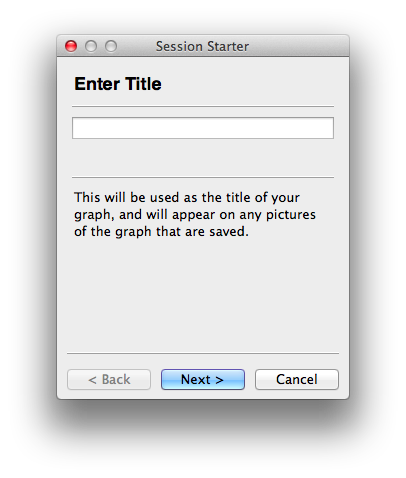
\includegraphics[width=\textwidth]{images/wizard_page_1.png}
        \caption{Wizard title chooser page}
        \label{fig:page_1}
    \end{subfigure}
    \begin{subfigure}[b]{0.4\textwidth}
        \centering
        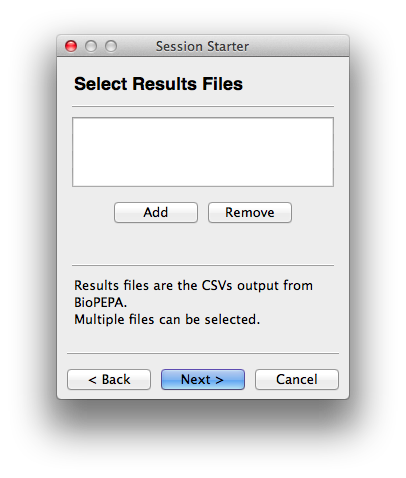
\includegraphics[width=\textwidth]{images/wizard_page_2.png}
        \caption{Wizard results selector page}
        \label{fig:page_2}
    \end{subfigure}

    \begin{subfigure}[b]{0.4\textwidth}
        \centering
        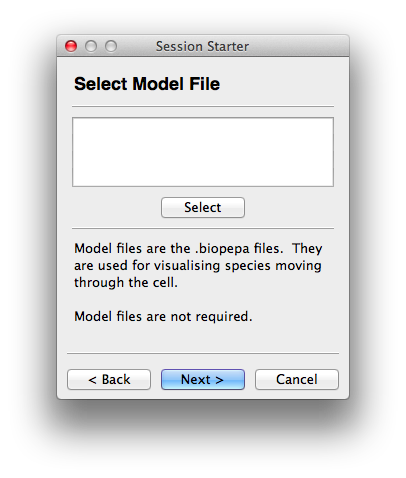
\includegraphics[width=\textwidth]{images/wizard_page_3.png}
        \caption{Wizard model selector page}
        \label{fig:page_3}
    \end{subfigure}
    \begin{subfigure}[b]{0.4\textwidth}
        \centering
        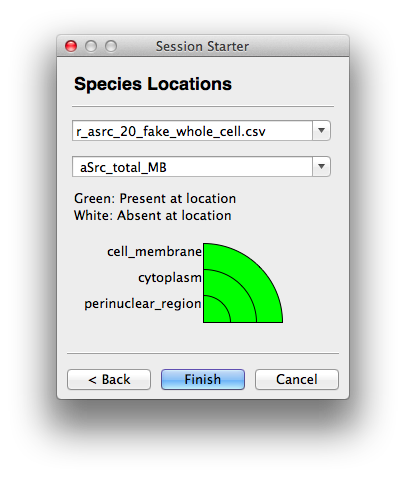
\includegraphics[width=\textwidth]{images/wizard_page_4.png}
        \caption{Wizard model viewing page}
        \label{fig:page_4}
    \end{subfigure}
    \caption{The session wizard that guides a user when setting up a session.}
    \label{fig:session_wizard}
\end{figure}

Form validators are used on the title fields and results fields.  The validators ensure that a title and at least one results file are included.  This stops the user from creating an invalid session.  There is also help text on each page of the wizard instructing the user on what actions they should take.

The model viewer page in Figure~\ref{fig:page_4} is similar to the cell cross-sections used in animation~\ref{sec:animation}.  There are two drop down boxes.  These drop down boxes control what is displayed in the cell cross-section.  Species in files can be selected.  The cell cross-section displays which compartments in the cell the species is present in.  The compartments are parsed from the model file.  This means that the model file is a requirement for model viewing and cell level animation.  This cell cross-section has replaced the previous model visualisation.  This model visualisation has two purposes. First, the user can sanity check that they have matching results and model files.  If a section of the cell has been left white then it acts as a cue to the user: if they were expecting the species to be present at that location then they know something has gone wrong.  Second, they can see how the model is structured.  The sections of the cell are labelled allowing the user to know what areas of the cell a species is present in.  This will hopefully increase their confidence with visualising and analysing the results from the models. Before the compartments were parsed from the model file automatically there was an user unfriendly system where the user had to input where in the cell a species is.  This was time consuming, difficult to use, and quite brittle.  At the time it assumed that there would be three compartments for every species, which is not a valid assumption.


\subsection{Matplotlib is Slow}

matplotlib is the de facto standard for graphing in Python this, amongst other reasons (detailed in the MPP report), led to it being chosen for the graph visualisations in the project.  When features such as plotting the intensity of the gradient were added matplotlib was pushed to its limits as it was being asked to plot hundreds of lines.  It was discovered that matplotlib is not optimised for speed, it is instead optimised for producing graphs of a publication standard.  This poses a dilemma: researchers want to be able to generate quality graphs, whilst the tool wants to offer real time interactivity and customisation.  There are tweaks that can be applied to make matplotlib be faster. There are also alternative graphing libraries that could be considered.  Threading was also looked into but caused segmentation faults.

\tdi{Became more noticable once collaboration was added and things were being redrawn more}


\subsection{Change how the visualisation is calculated}
Currently the visualisation is stored as a snapshot of the entire state.  The undo functionality is built around taking copies of this snapshot. When the visualisations are being displayed the \ac{UI} components look at this single snapshot.  Making copies of a large snapshot is not a cheap operation.  A more efficient approach would be to store operations.  To draw the latest visualisation the tool would simply traverse this list from the start.  Undoing an action would simply then be removing the last operation.
